\documentclass[10pt,a4paper,sans]{moderncv}
\moderncvstyle{banking}
\moderncvcolor{blue}
\usepackage[scale=0.90,top=0.7cm,bottom=0.7cm]{geometry}

% Encodage et accents
\usepackage[utf8]{inputenc}
\usepackage[T1]{fontenc}
\usepackage[french]{babel}
\usepackage{lmodern}
\usepackage{textcomp}
\usepackage{cmap}

\usepackage{enumitem}
\usepackage{fontawesome5}
\usepackage{graphicx}
\usepackage{tikz}

% Réduction espace entre sections
\renewcommand{\sectionskip}{\medskip}

% Puces personnalisées
\newcommand{\ringbullet}{%
  \tikz[baseline=-0.1ex]{
    \draw[color1, line width=0.8pt] (0,0) circle (0.08cm);
    \fill[color1] (0,0) circle (0.03cm);
  }
}
\setlist[itemize]{
    label=\ringbullet,
    leftmargin=1.2em,
    itemsep=0pt,
    topsep=0pt,
    parsep=0pt
}

\renewcommand{\cvtag}[1]{%
  \tikz[baseline]\node[anchor=base,draw=TagColor!40,rounded corners,inner xsep=1ex,inner ysep =0.75ex,text height=1.5ex,text depth=.25ex]{#1};
}

% En-tête personnalisé
\newcommand{\makeleftheader}{%
\begin{tikzpicture}[remember picture,overlay]
  \node[anchor=north east,inner sep=5pt] at ([xshift=-1cm,yshift=-0.5cm]current page.north east) {
    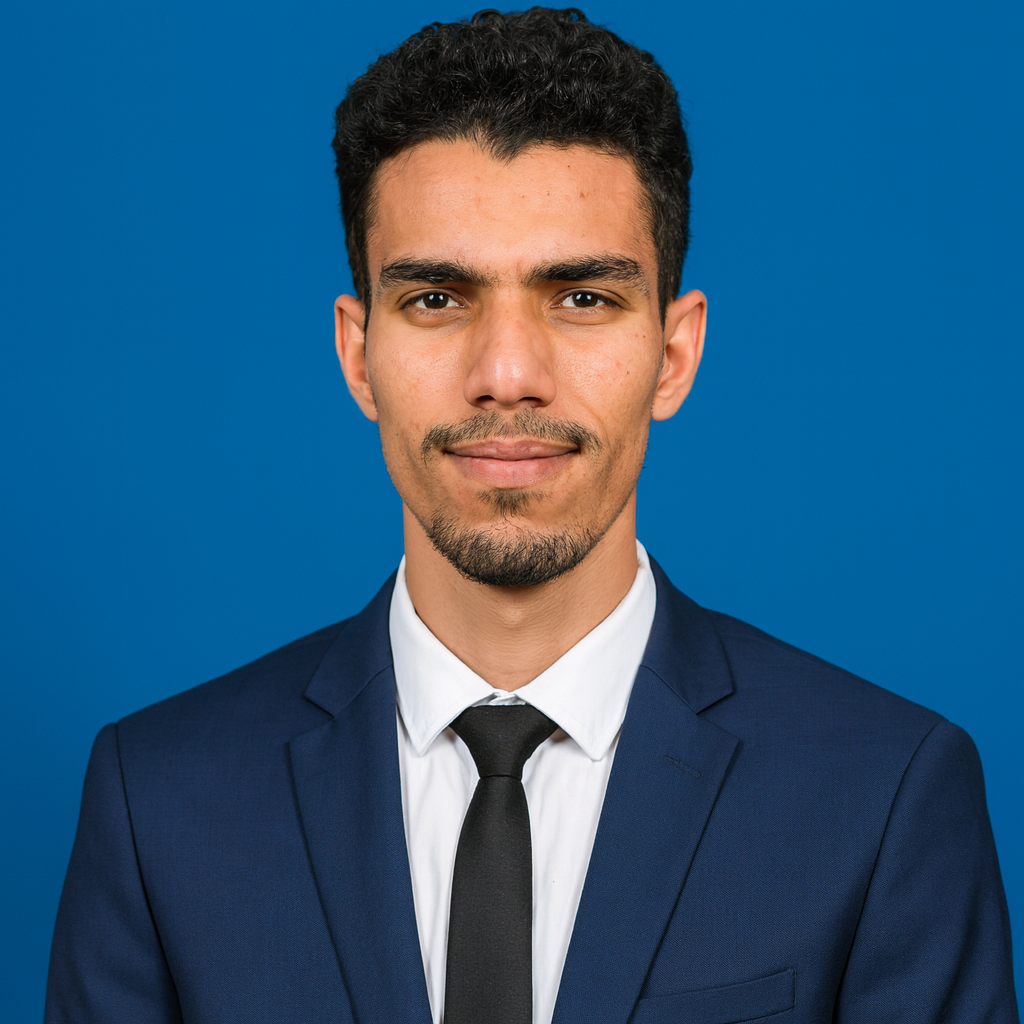
\includegraphics[width=2.8cm]{mouad.png}
  };
    
  \node[anchor=north west,inner sep=0pt] at ([xshift=1cm,yshift=-1cm]current page.north west) {
    \begin{minipage}{0.95\textwidth}
      \raggedright
      {\Huge\color{color1}\textbf{AIT AYACH MOUAD}} \\[0.5em]
      {\Large\color{color2}Ingénieur IA \& Data Science} \\[1em]
      
      \faPhone\ +33 6 12 61 75 97 \quad
      \faEnvelope\ mouadaitayach@gmail.com \quad
      \faLinkedin\ Mouad Ait Ayach \quad
      \faMapMarker\ Paris, France \\
      \faCar\ Permis B \quad
      \faMapMarker\ Mobile en France
    \end{minipage}
  };
\end{tikzpicture}
\vspace{2cm}
}

\begin{document}
\makeleftheader

\section{PROFIL}
\small{{{PROFIL}}}

\section{EXPÉRIENCES PROFESSIONNELLES}
{{EXPERIENCES}}

\section{FORMATION}
\cventry{2024 — 2025}{Master M2 - Knowledge integration in mechanical production, option : conception, industrialisation et innovation} {Arts et Métiers ParisTech}{France}{}{}
\cventry{2022 — 2025}{Cycle d'ingénieur filière Intelligence Artificielle \& Data Science}{Arts et Métiers Meknès}{Maroc}{}{}
\cventry{2020 — 2022}{Classes préparatoires intégrées}{Arts et Métiers Meknès}{Maroc}{}{}

\section{PROJETS ACADÉMIQUES}
{{PROJETS}}


\section{COMPÉTENCES}
{{COMPETENCES}}

\vspace{0.5cm}
\begin{minipage}[t]{0.3\textwidth}
\section{LANGUES}
\cvitem{}{Français — courant}
\cvitem{}{Arabe — Langue maternelle}
\cvitem{}{Anglais — courant}
\end{minipage}
\hfill
\begin{minipage}[t]{0.6\textwidth}
\section{RÉALISATIONS}
\cvitem{}{2\up{e} prix Innov’am – LafargeHolcim (projet de déchiqueteur industriel)}
\cvitem{}{Chef d’événement Mécaday – 1\up{re} édition}
\end{minipage}

\end{document}
